\documentclass[a4paper]{scrartcl}
\usepackage{fontspec}
\usepackage{graphicx}  
\usepackage[hmargin=28.8mm,vmargin=30mm]{geometry}     
\usepackage{dwmpcode}
\setcounter{secnumdepth}{1}
\overfullrule2pt
\begin{document}

\section{Moorish}

These designs are largely taken from the chapter on Moorish tiling patterns in Owen
Jones' \textit{Grammar of Ornament}, 1856. The section names are all mine.  Each file inputs
\mpl{jones-colors.mp}, which defines the six colours used as follows:
$$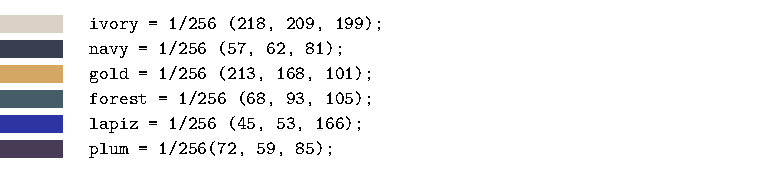
\includegraphics{jones-color-swatches}$$

\bigskip\noindent
Many of the patterns use regular polygonal stars, which are drawn by this macro:
\smallmpexternal[xleftmargin=0pt]{jones-generic-star.mp}
\noindent
The parameter $r$ is the radius of the star; $n$ and $s$ determine the shape, like
this:
$$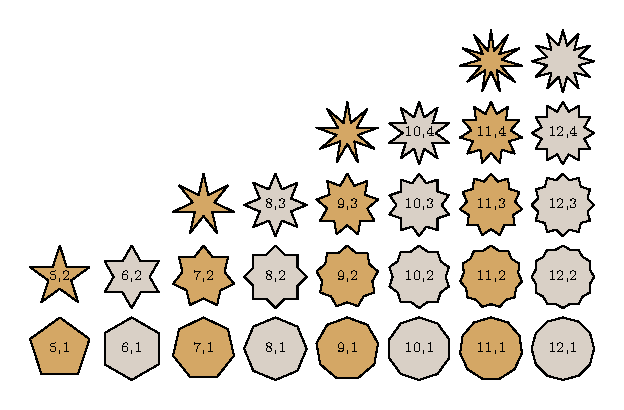
\includegraphics{jones-star-sampler}$$

\bigskip\noindent
Most of the patterns in the following pages are laid out on a square grid, 
but the last three use a triangular grid.

\subsection{Bats}
$$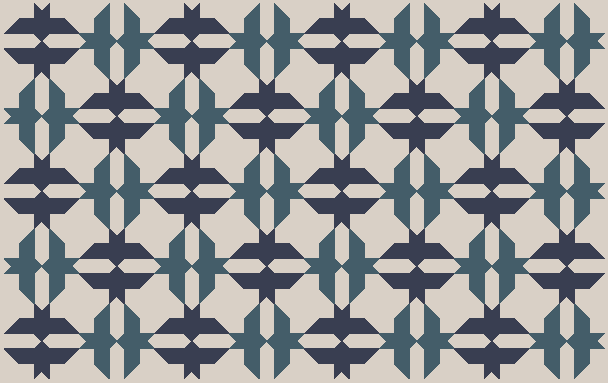
\includegraphics{jones-bats}$$
\smallmpexternal[firstline=7,lastline=22,xleftmargin=0pt]{jones-bats.mp}

\subsection{Carré}
$$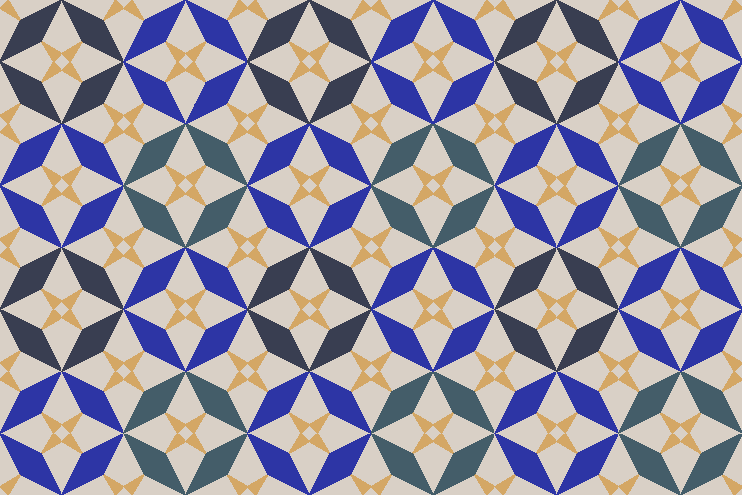
\includegraphics{jones-carre}$$
\smallmpexternal[firstline=7,lastline=33,xleftmargin=0pt]{jones-carre.mp}

\subsection{Cross}
$$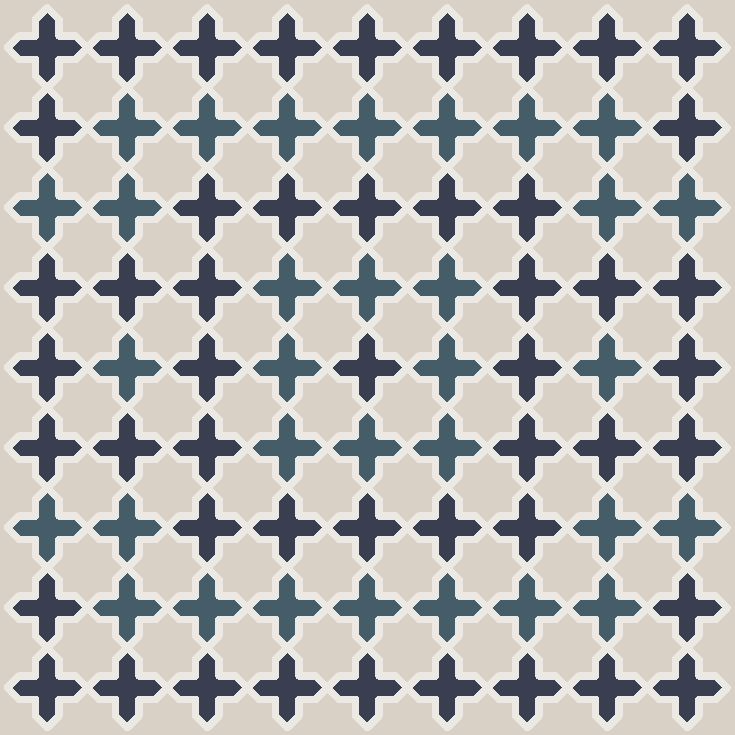
\includegraphics{jones-cross}$$
\smallmpexternal[firstline=7,lastline=28,xleftmargin=0pt]{jones-cross.mp}

\subsection{Lifebelt}
$$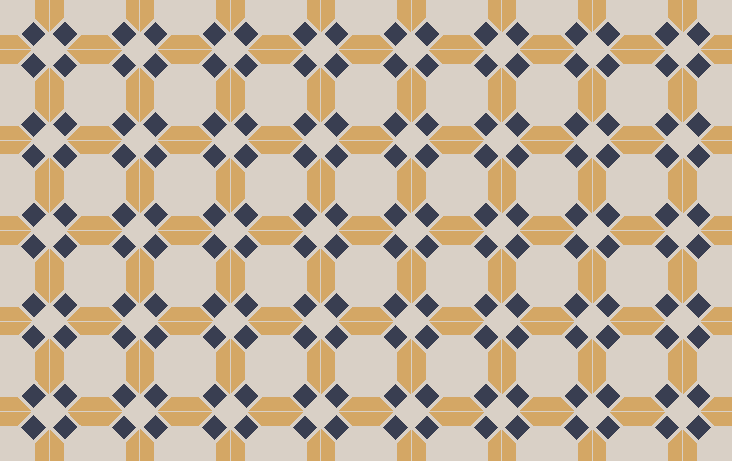
\includegraphics{jones-lifebelt}$$
\smallmpexternal[firstline=7,lastline=34,xleftmargin=0pt]{jones-lifebelt.mp}

\subsection{Octa-star}
$$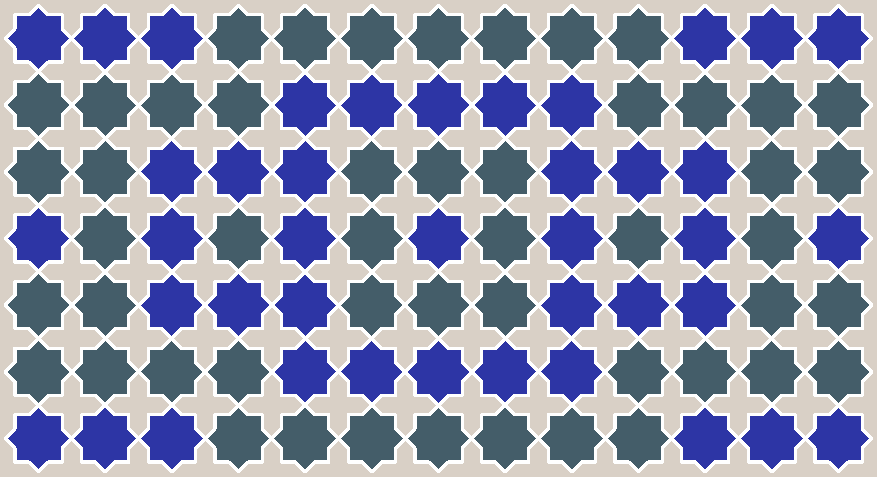
\includegraphics{jones-octa-star}$$
\smallmpexternal[firstline=8,lastline=21,xleftmargin=0pt]{jones-octa-star.mp}

\subsection{Quad}
$$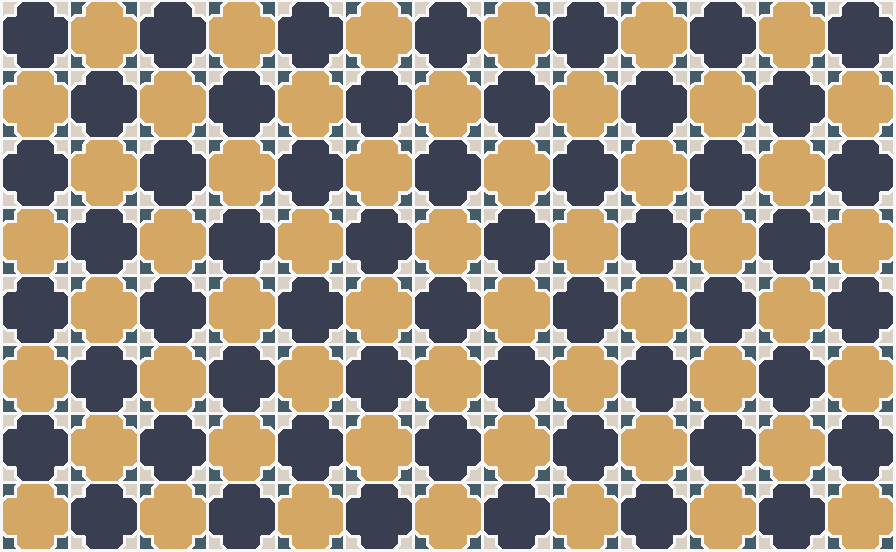
\includegraphics{jones-quad}$$
\smallmpexternal[firstline=7,lastline=33,xleftmargin=0pt]{jones-quad.mp}

\subsection{Rosette}
$$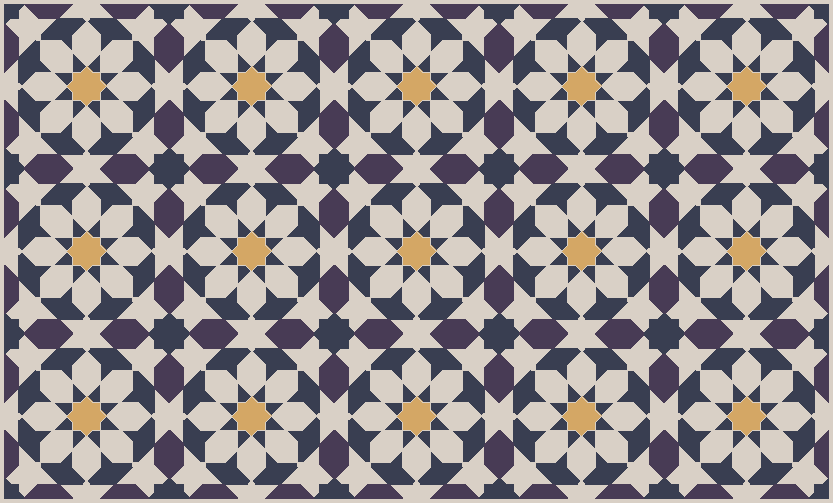
\includegraphics{jones-rosette}$$
\smallmpexternal[firstline=8,lastline=40,xleftmargin=0pt]{jones-rosette.mp}

\subsection{Scotch}
$$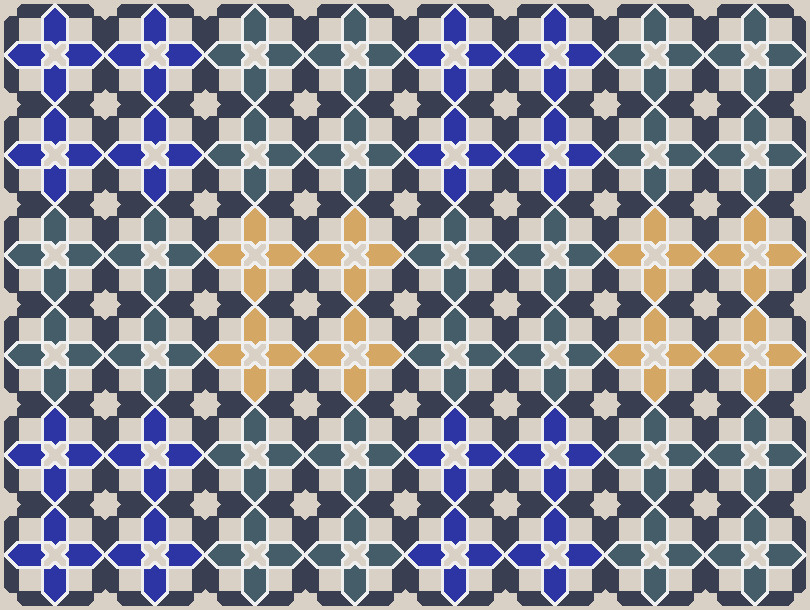
\includegraphics{jones-scotch}$$
\smallmpexternal[firstline=7,lastline=35,xleftmargin=0pt]{jones-scotch.mp}

\subsection{Star-flower}
$$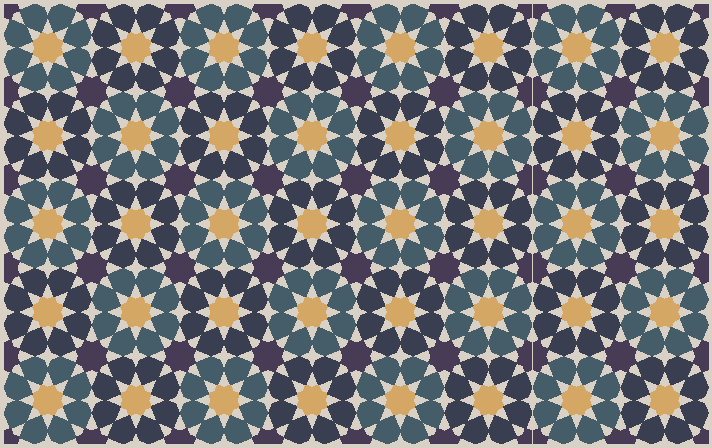
\includegraphics{jones-star-flower}$$
\smallmpexternal[firstline=8,lastline=41,xleftmargin=0pt]{jones-star-flower.mp}

\subsection{Sun}
$$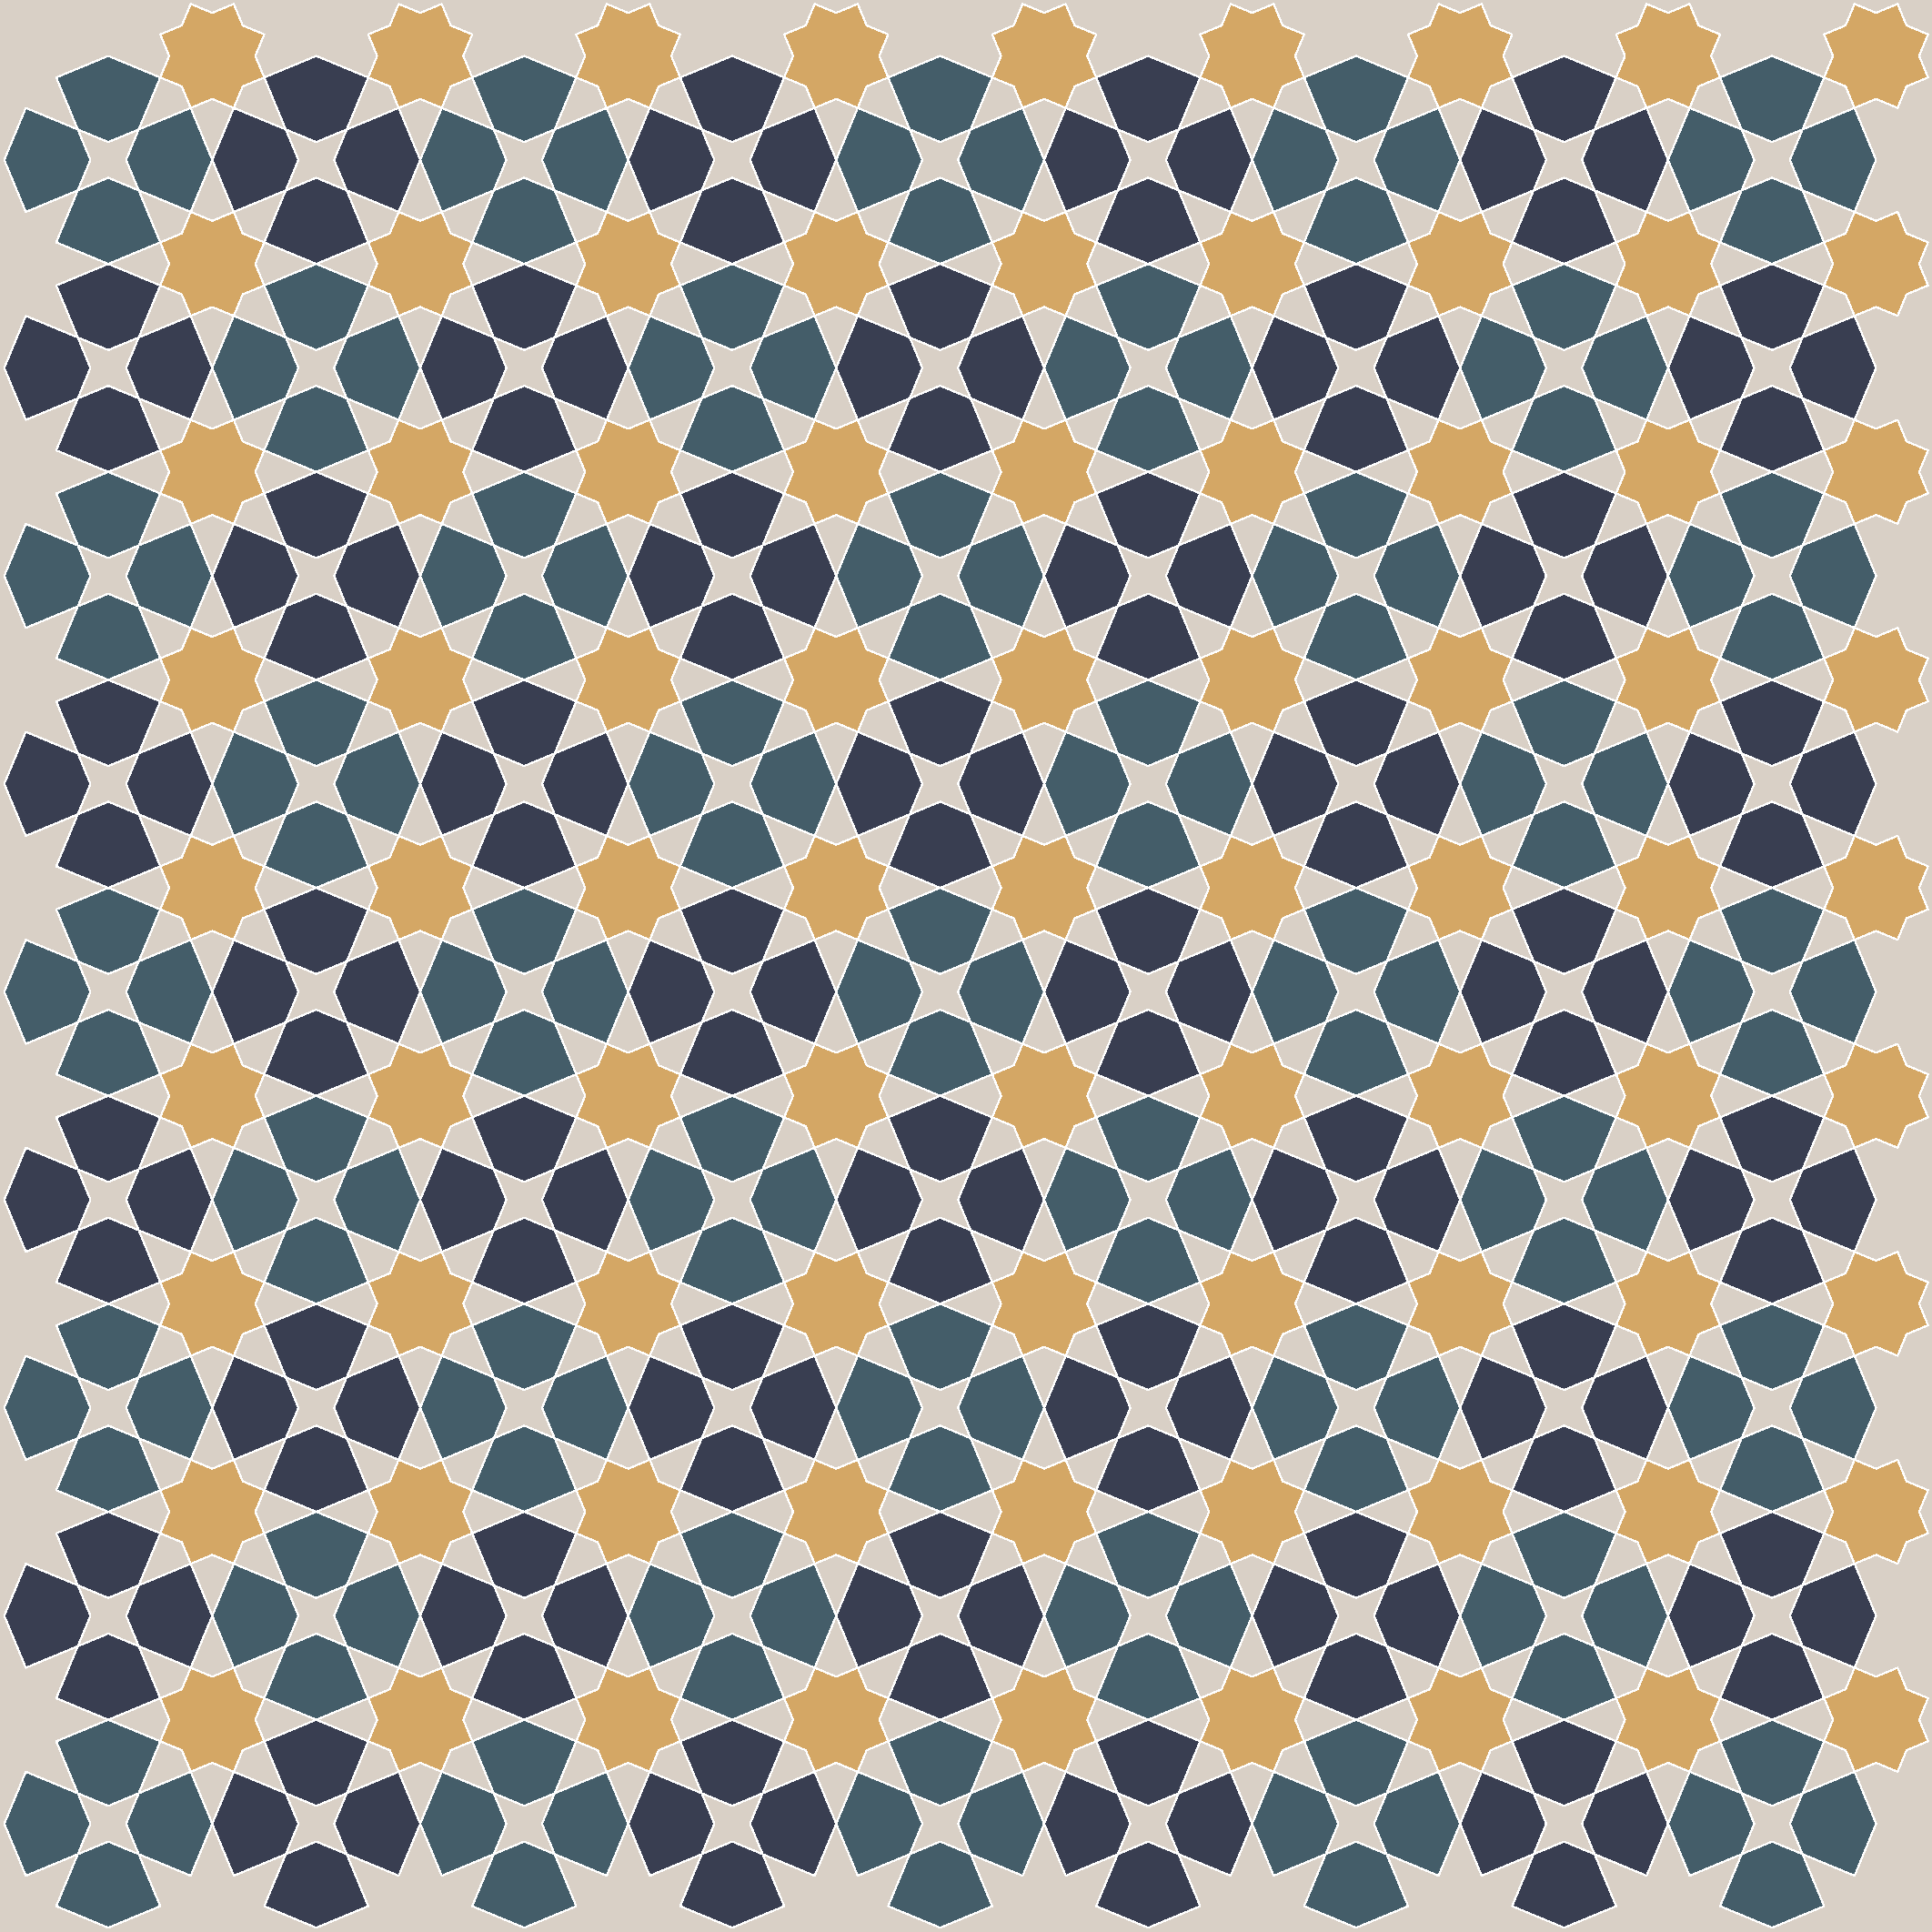
\includegraphics{jones-sun}$$
\smallmpexternal[firstline=8,lastline=41,xleftmargin=0pt]{jones-sun.mp}

\subsection{Tack}
$$
\includegraphics{jones-tack}$$
\smallmpexternal[firstline=7,lastline=29,xleftmargin=0pt]{jones-tack.mp}

\subsection{Hex-star}
$$
\includegraphics{jones-hex-star}$$
\smallmpexternal[firstline=7,lastline=37,xleftmargin=0pt]{jones-hex-star.mp}

\subsection{Twelve-and-nines}
$$\includegraphics{jones-twelve-nines}$$
\smallmpexternal[firstline=8,lastline=30,xleftmargin=0pt,xrightmargin=-60pt]{jones-twelve-nines.mp}

\vfill
\rightline{continued on next page \dots} 
\newpage
\noindent \dots from previous page\par\vfill
\smallmpexternal[firstline=32,lastline=69,xleftmargin=0pt,xrightmargin=-60pt]{jones-twelve-nines.mp}

\subsection{Twelve-pointers}
$$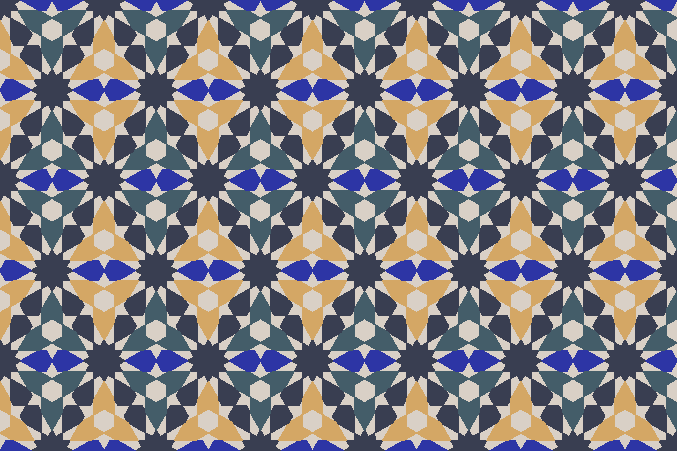
\includegraphics{jones-twelve-pointers}$$
\smallmpexternal[firstline=8,lastline=42,xleftmargin=0pt]{jones-twelve-pointers.mp}

\end{document}

